\section{Government \& Binding}
{\tiny Transformational Grammar and its subsequent incarnations (such as
Government and Binding Theory and Minimalism) were developed by
Noam Chomsky}\\
{\tiny The different implementations of Chomskyan theories are often grouped under the heading Generative Grammar, it comes from the fact that phrase structure grammars and the augmented frameworks that were suggested by Chomsky can generate sets of well-formed expressions }\\
\scriptsize{additional symbols:}\\ {\tiny C: Complementizer (subordinating conjunctions such as "that")\\
I: Finiteness (as well as Tense and Mood)\\
D: Determiner (article, demonstrative)
}\\
\scriptsize{projection levels} {\tiny X0: symbol that leads to the terminal symbol\\
X': intermediate projection \\
XP: highest projection (X'')
}\\
\scriptsize{Inflectional symbol INFL} {\tiny e.g. will, -s \\
both auxiliary and non-auxiliary constructions can be captured by the same underlying tree structure\\
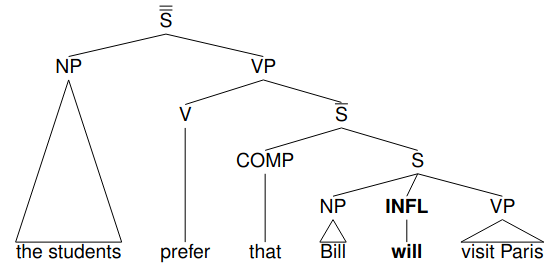
\includegraphics[scale=0.2]{infl.png}\\
problem: missing inflections, irregulars, language diversity\\
a structural analysis template that was developed for English}\\
\scriptsize{Deep Structure} {\tiny e.g. INFL VP}\\
\scriptsize{Surface Structure} 
{\tiny e.g. visit-s}\\
\scriptsize{CP and IP} 
{\tiny instead of S symbol, Complementizer Phrase and Inflectional Phrase as layers above the verb phrase\\
IP symbol essentially replaces the starting symbol S in GB analyses, the subject is considered the specifier of the IP, and the object is the complement of the IP\\
CP is yet another level above the VP, relevant when a complementizer is used, but also for other syntactic phenomena}\\
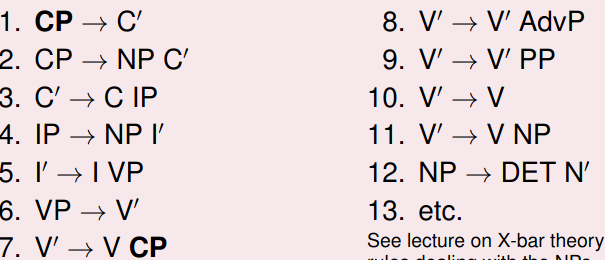
\includegraphics[scale=0.2]{cp-ip-rules.png}\\
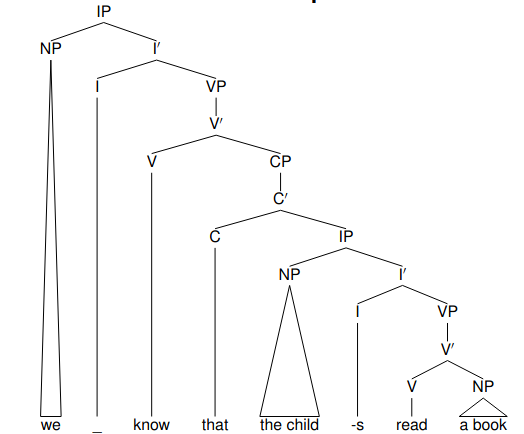
\includegraphics[scale=0.25]{GB_tree.png}\\
\scriptsize{Movement} 
{\tiny the verb moves up to the affix}\\
\scriptsize{Trace} 
{\tiny when an element moves into another position in the tree, it leaves a trace in the position where it was before}\\
\scriptsize{Pros} 
{\tiny Formulates a highly abstract and general template (D-Structure) which can be used to model all types of sentences and syntactic phenomena (at least aims to)}\\
\scriptsize{Cons} 
{\tiny requires many complicated mechanisms (movement, empty elements, case assignments...) to derive the set of possible sentences; lack of precise formulizations of these mechanisms has resulted in GB (and other Mainstream Generative Grammar approaches) being largely ignored by computational linguists}
\subsection*{Government}
{\tiny used in connection with case assignment between an I (e.g.will) and its specifier (e.g. the subject in nominative case), and between a verb head (e.g. read) and its complement (e.g. a book) in accusative/dative case)}\\
\scriptsize{case principle} {\tiny V assigns objective case (accusative) to its complements if it bears structural case\\
When finite, INFL assigns case to the subject\\
prepostions assign cases to the NPs they head\\
every maximum projection (XP) that dominates the NP that receives Case also dominates the head that assigns it
}\\
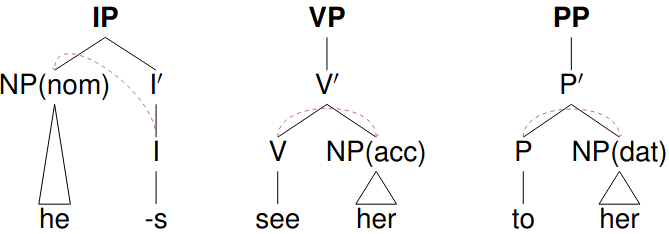
\includegraphics[scale=0.2]{case-assignment.png}\\
\scriptsize{Government} {\tiny alpha governs beta iff:\\
(i) alpha is a head, and \\
(ii) every XP that dominates alpha also dominates beta, and \\
(iii) every XP (other than IP) that dominates beta also dominates alpha\\
(dominate means a certain element is the mother-node or higher up in the tree of another element)
}\\
\scriptsize{problems} {\tiny unclear what exactly the relationship between case assignment and government is; case assignment can only work between some governor and a XP, unclear how this case then gets assigned to the elements further down the branches}
\subsection*{Binding}
{\tiny to determine when a reflexive anaphor, e.g. herself, is used instead of one of the pronouns she or her}\\
\scriptsize{Binding} {\tiny alpha binds beta iff:\\
(i) alpha does not dominate beta, \\
(ii) the mother-node that dominates alpha also dominates beta \\
(iii) alpha and beta are coindexed\\
(the first two clauses simply mean that alpha c-commands all categories below its own mother node)
}\\
\scriptsize{principles of binding theory} {\tiny (A) Pronouns (non-reflexive) must not be bound in their governing Inflectional Phrase (IP)\\
(B) reflexive Pronouns must be bound in their governing Inflectional Phrase (IP)\\
(C) Full NPs (aka denoting expressions) must not be bound\\
(accounts for the fact that the same full NP cannot be used again in ta single sentence, but have to be represented by a pronoun)\\
every maximum projection (XP) that dominates the NP that receives Case also dominates the head that assigns it
}\\
\scriptsize{problems} {\tiny several possible usages of reflexive and non-reflexive
pronouns do not conform to the rules of Binding Theory; no clear rules which NPs and pronouns are co-indexed.}
\subsection*{Syntactic Phenomena}
\scriptsize{T model} {\tiny (called by its shape when you invert it), a schematic representation of all the underlying processes assumed for generating well formed sentences in GB theory
}\\
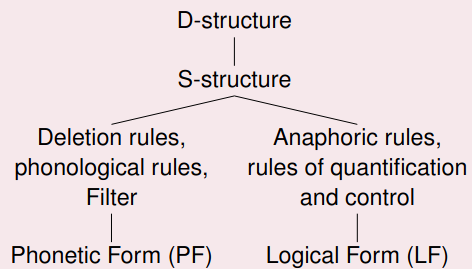
\includegraphics[scale=0.2]{t-model.png}\\
\scriptsize{D-Structure} {\tiny the underlying template or mould that is used to build all grammatical sentences in a given language}\\
\scriptsize{S-Structure} {\tiny derived by transformations which allow to move elements around and reassign cases\\
surface structure is not necessarily the actual string or phonemes that you might read or hear, deletions and phonetic rules might still apply}\\
\scriptsize{Deletion rules} {\tiny can be applied to the surface structure, indicated by underscores}\\
\scriptsize{Phonetic Form} {\tiny regular changes to the surface structure, e.g. wants to->wanna}\\
\scriptsize{Logical Form} {\tiny only marginally discussed, through binding theory (anaphora resolution)}\\
\scriptsize{Yes/No questions}\\
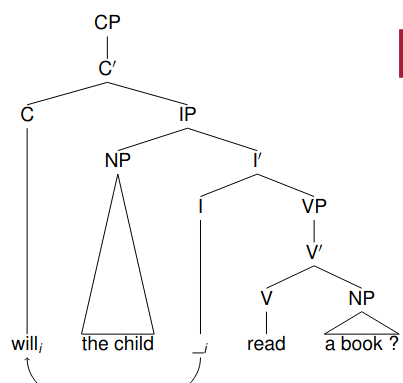
\includegraphics[scale=0.2]{yes-no.png}\\
\scriptsize{Wh-Questions}\\
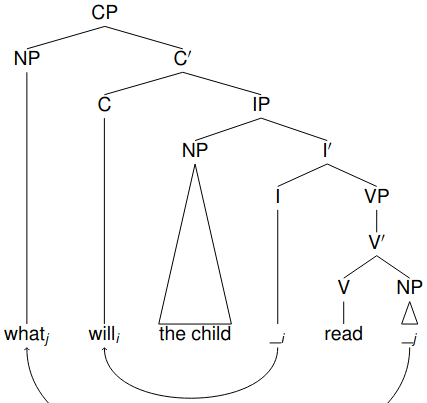
\includegraphics[scale=0.2]{what.png}\\
\scriptsize{Verb position} {\tiny verb position can be handled by flexibly changing the order of elements in the rewrite rules for IP and VP}\\
\scriptsize{parameters} {\tiny introduced to explain how variation (e.g. in verb position) across languages of the world can be explained against the backdrop of the same underlying deep structure}\\
\scriptsize{Fronting} {\tiny fronted element moved into positions of higher level phrases (CP and IP), like wh-movement or movement of auxiliaries in questions}\\
\scriptsize{Passive} {\tiny the same underlying deep structure as active constructions}\\
\scriptsize{Active(D-Structure)}\\
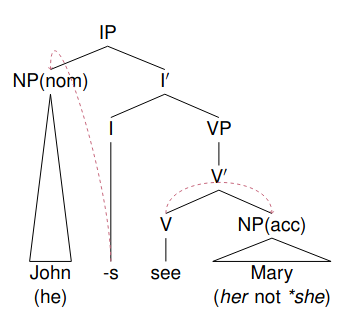
\includegraphics[scale=0.25]{GB_active.png}\\
\scriptsize{Passive(S-Structure)}\\
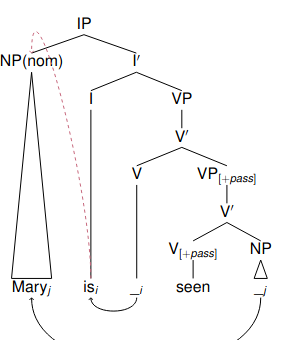
\includegraphics[scale=0.25]{GB_passive.png}\\
\scriptsize{Ditransitives} {\tiny problematic for GB analysis, need an additional recursive rule V'->V' NP\\
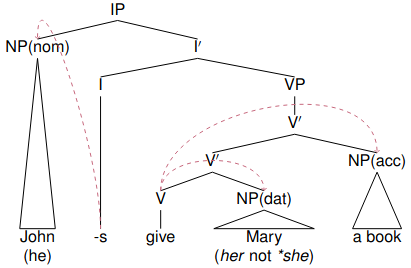
\includegraphics[scale=0.2]{ditransitive.png}\\
Problems: implies a verb can take arbitrarily large number of complements; run into problems with Binding Theory when reflexive pronouns are used}
